\documentclass[../../lecture_notes.tex]{subfiles}
\begin{document}


Schedulers can work on multiple levels:
\begin{enumerate}
\item long-term scheduler \\
	which processes should be admitted to OS?
	\begin{itemize}
	\item look at return value of fork()
	\item if fork() < 0, denied by OS
	\end{itemize}
\item medium-term scheduler \\
	which processes reside in RAM?
\item short-term scheduler \\
	which threads get to run on the limited number of CPUs
\end{enumerate}


A process can be in one of three states:
\begin{enumerate}
\item \term{Running} $\coloneqq$ executing instructions on a processor
\item \term{Ready} $\coloneqq$ ready to run but waiting on OS
\item \term{Blocked} $\coloneqq$ waiting on another event
\end{enumerate}


In addition to these three, there are the edge cases of:
\begin{enumerate}
\item \term{Initial} $\coloneqq$ just created, environment not set up
\item \term{Final/Zombie} $\coloneqq$ process is complete but hasn’t been cleaned up yet 
\end{enumerate}

Moving from ready to running is called being \term{scheduled}.Moving from running to ready is called being \term{de-scheduled}. The act of scheduling is assigning CPUs to threads. Each instruction pointer requires a CPU to run. This requires a harmony of hardware and software
    

Determining how to schedule is easy when we have enough CPUs, but what do we do if there are more threads than CPUs?

We need a few things to answer this
\begin{itemize}
\item Theory: scheduling policy
\item Practice: Scheduling and Dispatch Mechanisms
\end{itemize}


Tiny gaps where neither thread is executing are called \term{context switches}, and are done by the OS. These can be timed in two broad ways:
\begin{enumerate}
\item Cooperative Scheduling $\coloneqq$a thread “volunteers” to give up its CPU with syscalls
\item Preemptive Scheduling $\coloneqq$ the OS preempts threads every time slice
    \begin{itemize}
	\item this is cheap and easier on the OS
	\item this is common in IOT/embedded systems
	\item short slice = less efficient
	\item long slice = long wait
	\end{itemize}
\end{enumerate}


How do threads “volunteer”?
\begin{lstlisting}
#include <sched.h>
int sched_yield(void);
\end{lstlisting}


We can use this to make waiting on a device more efficient:
\begin{lstlisting}
// we can bust wait
while(isbusy(device)) continue;
// we can poll, which is still ineffecient (but better)
while(isbusy(device)) sched_yield()
// or we can block, telling kernel to wake it when the condition is met
while(isbusy(device)) wait_until_ready()
\end{lstlisting}


The Linux scheduler runs the following algorithm:
\begin{lstlisting}
for (;;) {
	choose an unblocked thread
	load it into a CPU
	run it
	yield
	store state
	for each thread that has become ready
		unblock
}
\end{lstlisting}
    

This scheduler is completely terrible!  People have measured! But what did they measure?

\begin{center}
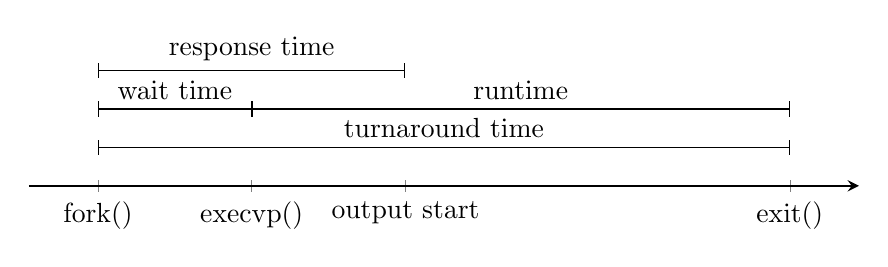
\begin{tikzpicture}
\begin{axis} [ 
	width=\linewidth, axis y line=none, ytick={}, axis x line=center, enlargelimits=true, axis line style=thick,
	xmin=0, xmax=9, ymin=0, ymax=2, axis equal,
	xtick={0, 2, 4, 9}, xticklabels={fork(), execvp(), output start, exit()}
]
\addplot[|-|, domain=0:9] {0.5} node[pos=0.5, above] {turnaround time};
\addplot[|-|, domain=0:2] {1.0} node[pos=0.5, above] {wait time};
\addplot[|-|, domain=2:9] {1.0} node[pos=0.5, above] {runtime};
\addplot[|-|, domain=0:4] {1.5} node[pos=0.5, above] {response time};
\end{axis}
\end{tikzpicture}
\end{center}


In addition, SEASNET screws us students over with a priority queue with priorities:
\begin{enumerate}
\item root
\item operations staff
\item students/faculty
\end{enumerate}

And each of these contains its own sub-scheduler and algorithm

Usually, priority 1 is the highest priority, but SEASNET uses the ides of \term{niceness}. If p1 has niceness x and p2 has niceness y > x, p2 will defer. users can raise a program’s niceness, but cannot lower it.

We can’t be too harsh though… there is a lot of complexity involved in \term{real-time systems}.


\subsection{Real-Time Scheduling}

This contains two types of deadlines:
\begin{itemize}
\item HARD:
	\begin{itemize}
	\item deadlines CANNOT be missed, $\implies$ performance = correctness
	\item predictability > performance, $\implies$ caches are the enemy
	\item use polling instead of interrupts, since polling controls test duration
	\end{itemize}
\item SOFT:
	\begin{itemize}
	\item a missed deadline is not necessarily a failure
	\item 2 scheduling options:
	\begin{enumerate}
	\item rate-monotonic scheduling $\coloneqq$ give a \% usage to job data streams
	\item earliest deadline first $\coloneqq$ can drop late requests when inundated. This allows one stream to monopolize the CPU. \\
	ex) Video Playback: Each frame is treated as its own request. When the connection is slow, the scheduler periodically drops frames; this is often imperceptible to humans
	\end{enumerate}
	\end{itemize}
\end{itemize}
                

Most real-life systems have both hard and soft real-time scheduling; this introduces a lot of complexity.  


\end{document}